\documentclass[a4paper, 12pt]{article}
\usepackage[utf8]{inputenc}
\usepackage[margin=3cm]{geometry}
\usepackage{natbib}
\usepackage{float}
\usepackage{graphicx}
\usepackage{fancyhdr}

\title{Measuring Language Ambiguity}
\author{Simon Schaefer}

\pagestyle{fancy}
\fancyhf{}
\rhead{Measuring Language Ambiguity}
\lhead{Simon Schaefer}
\rfoot{\thepage}

\begin{document}

\maketitle

Lobbying has impact on the legislation in modern democracies. However although this statement meets qualitatively approval, whether a larger amount of campaign contributions qualitatively leads to more ambiguous legislation is hardly analysed. Therefore the goal of the underlying project is to measure impact of campaign financing on the ambiguity of the resulting legislation, divided by several industry sectors.

\section*{Related Work and Theoretical Foundations}
Word embeddings have been shown to be unable to capture different meanings of a word, even if the meaning occurs in the same dataset. In fact different meanings have a negative impact on accurate semantic modeling as unrelated words that have a sense similar to different senses of the same word are pulled together, e.g. the word \textit{mouse} in Fig. \ref{fig:conflation_word_embedding}.

\begin{figure}[H]
\begin{center}
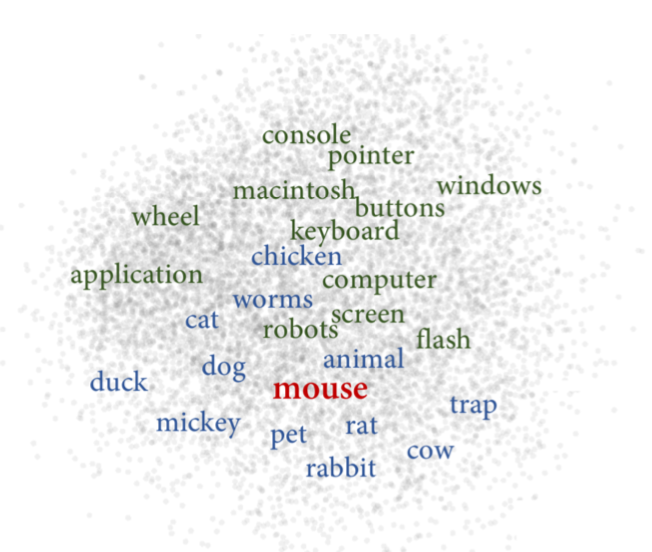
\includegraphics[width=6cm]{imgs/conflation_word_embedding}
\end{center}
\caption{Deflation and ambiguity of word embeddings \cite{word_to_sense_embedding}}
\label{fig:conflation_word_embedding}
\end{figure}

This problem can be solved by using sense embeddings instead, associating each word a category, so that words can be distinguished as being words of the same category (hypernymys) or of different categories. As \cite{word_to_sense_embedding} describes to construct sense embeddings there are two main paradigms, unsupervised and knowledge-based models. While unsupervised models (e.g. \cite{unsupervised_latent_vector_weighting}) induce different senses of a word by analysing its contextual semantics in a corpus, knowledge-based systems such as WordNet \cite{wordnet} are based on human-inputted senses of a word. As purposed by Pilehvar and Collier \cite{knowledge_based_page_rank}, DeConf, a personalized PageRank algorithm can be used to extend word embeddings by different senses (\textit{sense biasing words}), in order to maintain the euclidean order of the embedded space (deflation problem).

\begin{figure}[H]
\begin{center}
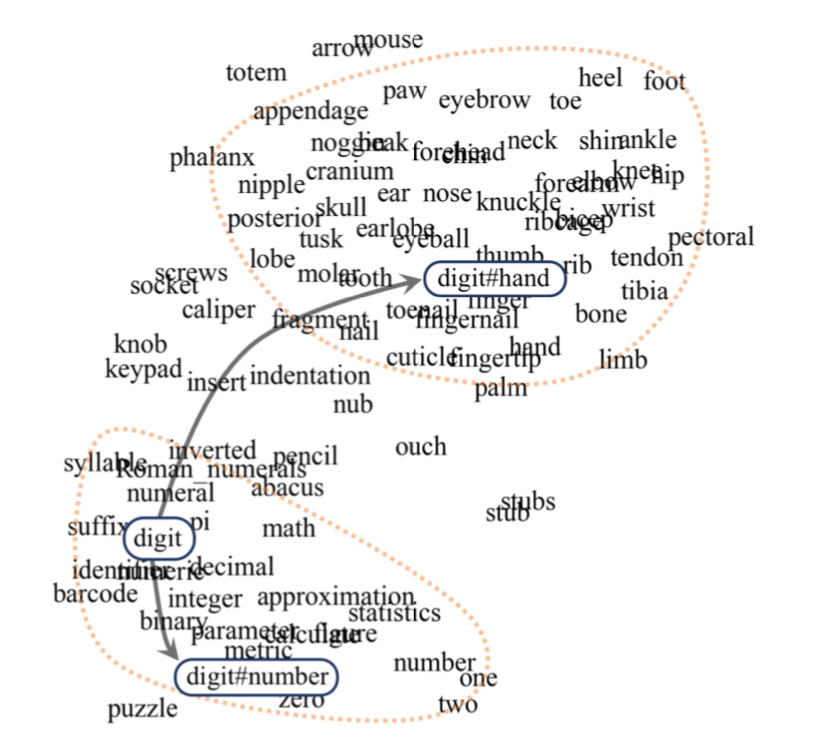
\includegraphics[width=6cm]{imgs/page_rank_embedding}
\end{center}
\caption{Sense Embeddings using DeConf algorithm \cite{knowledge_based_page_rank}}
\label{fig:page_rank_embedding}
\end{figure}

However, taking into account one word only and analyse the number of senses it has, instead of including contextual information to the analysis will not result in a well-performing scale for ambiguity, as demonstrated in the following example:

\begin{center}
My \emph{mouse} is broken, so I will buy another one.
\end{center}

Although the word \textit{mouse} has several senses (as shown in \ref{fig:conflation_word_embedding}), in the example above the sense is not ambiguous at all, as without doubt the \textit{computer mouse} is meant for the sentence to make sense. Taking the word combination \textit{mouse}+\textit{broken} the statement is not ambiguous anymore. For this reason in the underlying project the goal is to extend the sense embeddings technique presented above to 2-grams (noun+verb).

\section*{Approach}
In order to quantify ambiguity the number of ambiguous 2-grams should be counted, normalized for each bill. As described above 2-gram sense embeddings ascertained by an unsupervised learning technique using the page-rank algorithm purposed by Haveliwala \cite{topic_sensitive_page_rank} and Pilehvar et al. \cite{senses_to_texts}, as no groundtruth labels are existing for the \textit{sense} of 2-grams, can be used for this task. However, before the ambiguity model can be applied and succesfully trained, as shown in Fig. \ref{fig:overview_approach}, the bill's text data have to be preprocessed first (removing stopwords, stemming, convert to 2-grams, etc.).

\begin{figure}[H]
\begin{center}
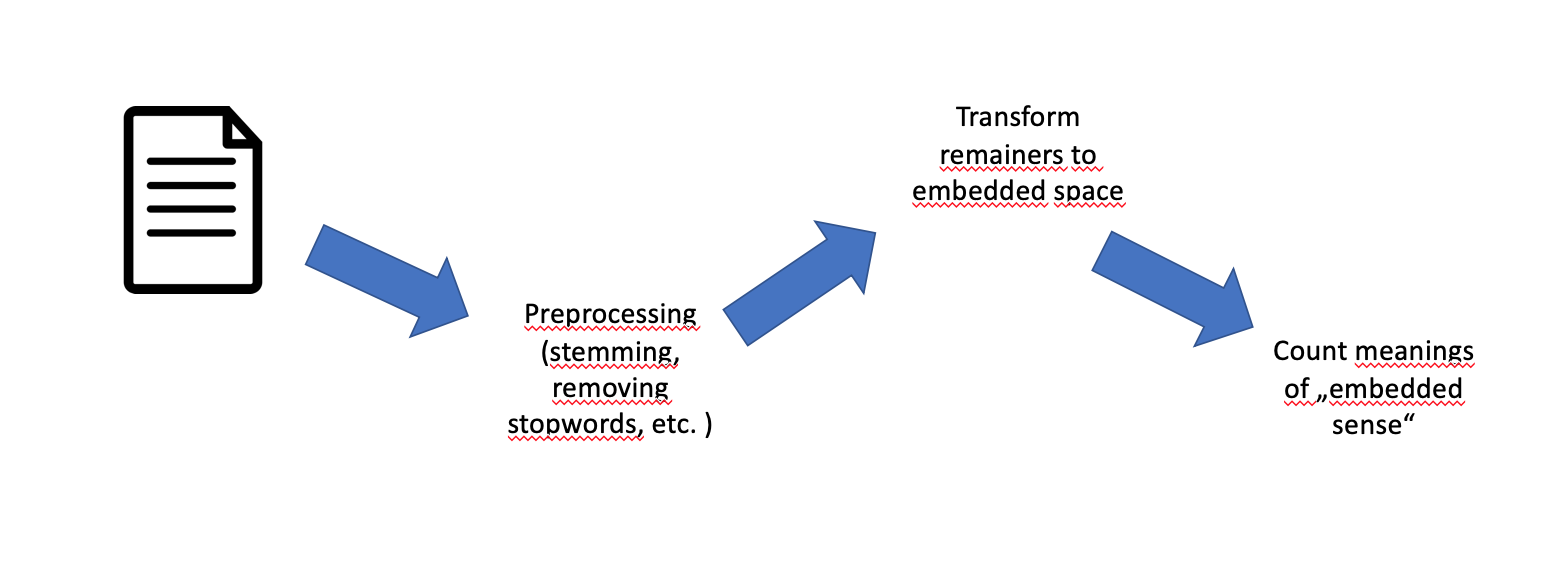
\includegraphics[width=10cm]{imgs/overview_approach}
\end{center}
\caption{Ambiguity Pipeline}
\label{fig:overview_approach}
\end{figure}

Next to determining the normalized level of ambiguity, each bill's text is clustered in one of several industry sectors using a Word2Vec model. \footnote{The exact cluster origin, i.e. the industries looked at, are still to be determined and depend on the occurence of various industry sectors in the law text.}. Having the industry sector, the US state and the normalized level of ambiguity assigned to each bill, ambiguity and contribution limit can be compared following a difference in differences (diff-in-diff) approach.

\section*{Datasets}
Two datasets are used, the first dataset, the US statue dataset from Ash as well as the campaign financial contribution dataset from Ash and Vannoni. Both dataset relate to all US states.

\begin{figure}[H]
\begin{center}
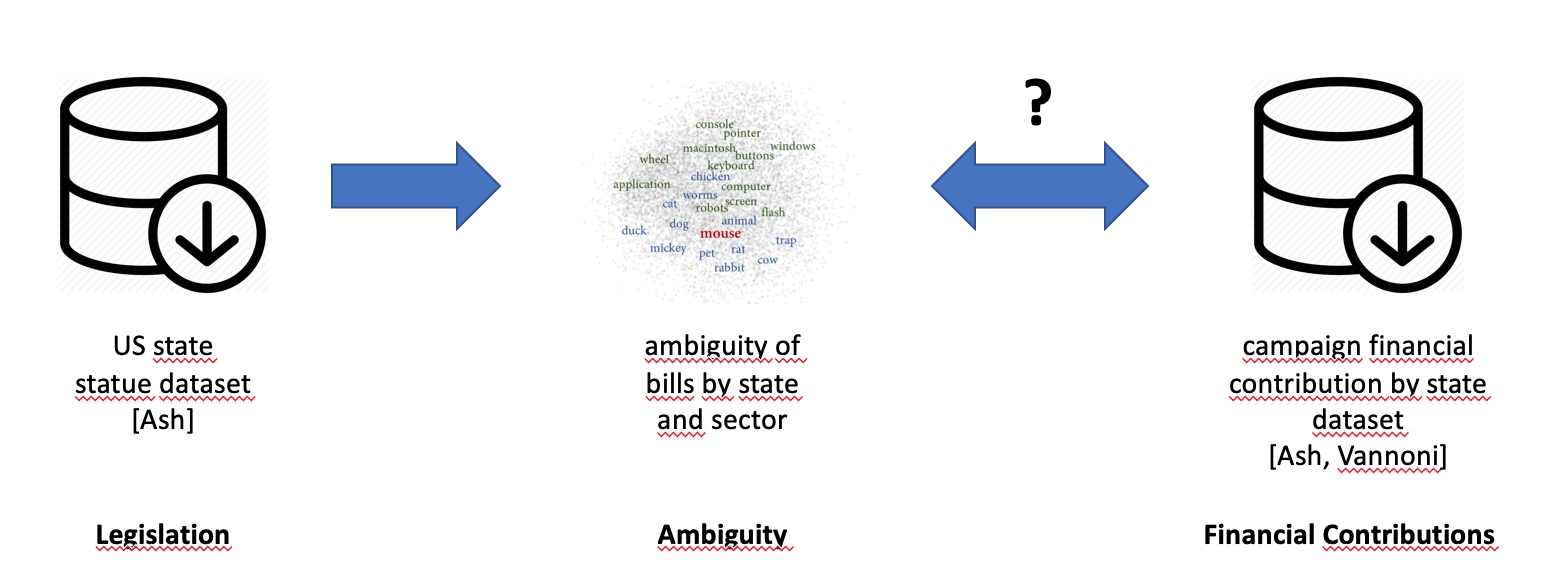
\includegraphics[width=10cm]{imgs/overview_datasets}
\end{center}
\caption{Overview of Datasets: financial contribution are compared with ambiguity
score by state and industry sector which is determined using the US statue
dataset}
\label{fig:overview_datasets}
\end{figure}

The US statue dataset contains bills for every US state voted upon in the time period from 1950 until recently, stating next to the bill's text several information about the formation and voting process. However, merely the text will be used.
\newline
The campaign financial contribution dataset contains the campaign contribution limits in each US state in between 1950 and 2000, as categorized data. This dataset can directly be used without the need of further preprocessing.
\newline
Both datasets are not publically available, however to still ensure the validity of the work next to the final correlation between ambiguity and financial contribution interim results will be published, such as the ambiguity measure and related sector of each considered US bill. To further improve reproducibility a pretrained model will be used for measuring ambiguity so that its performance is independent from the specific datasets used in this project. 

\section*{Roadmap/Timeline}

\begin{tabular}{c|p{10cm}}
Deadline & Description \\
\hline
07.06 & Definition of application (datasets) and already existing approaches
(language ambiguity) \\
23.06 & Preprocessing of US statue dataset including clustering the bills by
industry sector \\
07.07 & Implementation and training of ambiguity model on test data \\
21.07 & Apply ambiguity model to US statue dataset and comparing ambiguity results with campaign financial contribution datase by state and industry sector \\
17.08 & Report finished
\end{tabular}

\section*{Future Work}
In future work the same approach could be applied to data from outside of the US and differences in the impact of campaign contributions on the legislation between countries could be analysed. Also the language ambiguity model could be improved by extending it to even larger n-grams in order to avoid further \textit{artificial} ambiguity and further factor in the context.

\newpage
\bibliographystyle{plain}
\bibliography{references}

\end{document}
